%\newpage

\subsection{Specific Aim 2: Efficient high-order numerical methods for
large-scale simulations}
\label{subsec:specific_aim_2}
%\begin{figure}[h]
\begin{wrapfigure}[13]{r}{0.61\textwidth}
  \centering{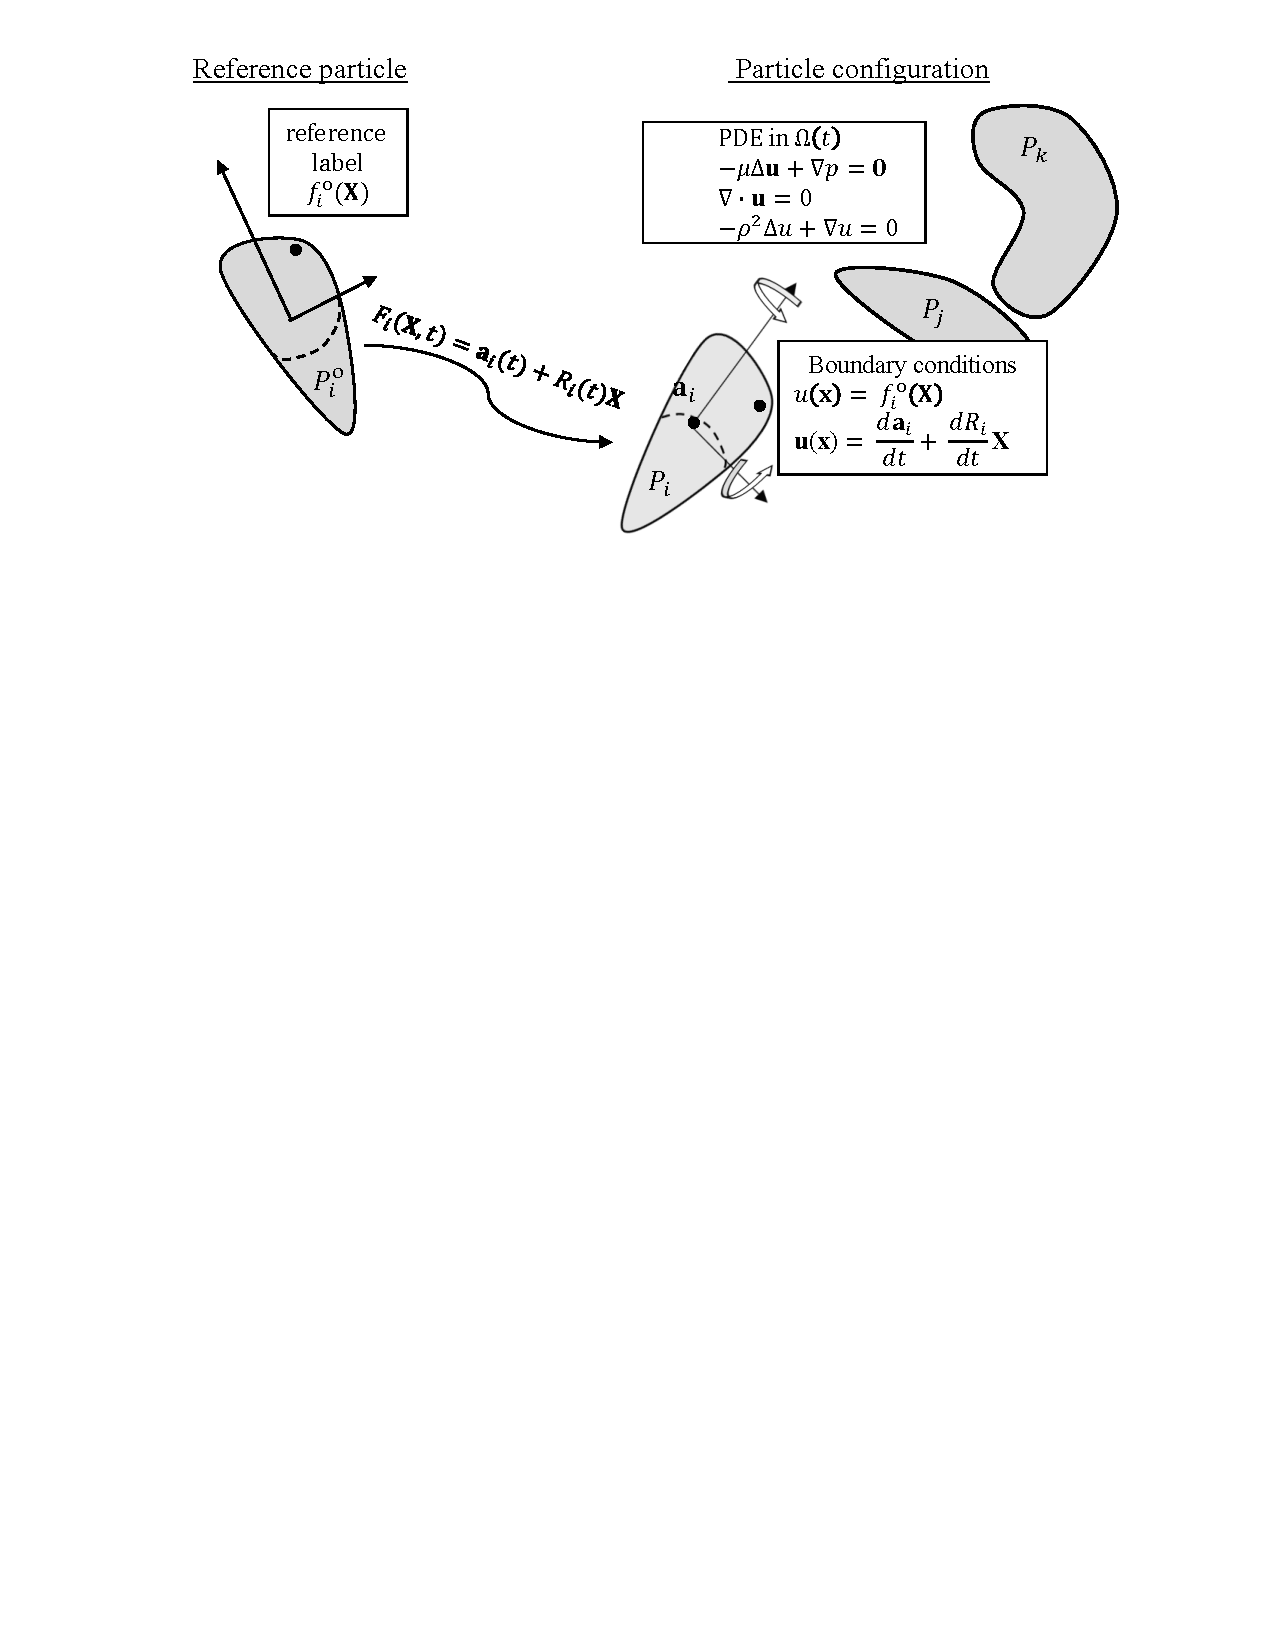
\includegraphics[width=0.61\textwidth]{Figures/domain.pdf}}
    \vspace{-20pt}
    \caption{\label{fig:flow_map} \footnotesize A suspension of 3D
    amphiphilic particles suspended in a solvent. The solvent satisfies
    the Stokes equations, and the hydrophobic forces depend on the
    solvent activity that satisfies the screened Laplace equation. The
    geometry is updated by solving the mobility problem.} 
\end{wrapfigure}
%\end{figure}
% ----------------------------------------------------------------------
Over the past decade, there has been an explosion of interest in
small-scale processes that utilize capillary forces, van der Waals
interactions, and thermal noise~\cite{Zhang2017}, to coordinate movement
and bind nano-legos in a solvent~\cite{Pandey2011, Leong2007,
Reynolds2019, Dasgupta2017, Siontorou2017}. Additionally, hydrodynamic
interactions are central to fabricate for complex microscopic
three-dimensional structures~\cite{Cho2010}. Hydrodynamic effects can
not be ignored since the rates of biological functions like fusion,
fission, and pore dynamics rely on viscous
dissipation~\cite{RYHAM20112929}.
%
In Specific Aim 2, we propose to develop efficient high-order numerical
methods to simulate dynamic assembly of particles under HAP potential in
a viscous solvent. 
%
%
%hydrodynamics effects by em
%particles in a solvent. 
%
% Results from these proposed numerical simulations will be useful to 
% Finally, coarse-grained and molecular
%dynamics theories include water either explicitly or implicitly in their
%models. 
%
%The immediate goal of the present proposal is to simulate
%vesicle bilayers in external flows, where the bilayers are represented
%by a self-assembled collection of rigid particles.
%
As described in~\eqref{eq:stokes} and illustrated in
Figure~\ref{fig:flow_map}, the solvent phase is modeled by the Stokes
equations for an incompressible viscous fluid, and these equations are
coupled to the screened-Laplace equation~\eqref{SL} through viscous and
hydrophobic stress balance. 
 
%While hydrophobic attraction causes the particles to self-assemble indepedently of the dissipation mechanism, the trajectories and
%equilibrium configurations depend on the fact that the particles travel through a viscous environment. 



The HAP model requires solving exterior Dirichlet problems for the
screened Laplace equation and the Stokes mobility problem at each time
step in complex domains such as in Figure~\ref{fig:domain}. If
discretizing these equations with stencil-based numerical methods, the
computational domain must be truncated, the fluid volume must be
discretized, and artificial boundary conditions must be imposed. The
artificial boundary conditions introduce additional error, and
discretizing the volume results in an excessively large system of
equations. Moreover, it is difficult to obtain high-order
discretizations when the boundary surfaces are irregular. Alternatively,
since we are solving constant-coefficient linear elliptic PDEs, its
solution can be represented with layer potentials
\begin{align}
  \label{eq:LP}
  u(\mathbf{x}) = \int_{\partial\Omega} K(\mathbf{x},\mathbf{y})
  \sigma(\mathbf{y})\,dS,
\end{align}
where $\sigma$ is an unknown density function, and
$K(\mathbf{x},\mathbf{y})$ is a derivative of the fundamental solution
of the PDE. By matching the prescribed boundary condition at
$\mathbf{x}_0 \in \partial\Omega$ with the limit of
equation~\eqref{eq:LP} as $\mathbf{x}\rightarrow \mathbf{x}_0$, a BIE
for the density function is formed. 

Numerical methods to solve BIEs have several advantages over their
PDE-based counterpart: by construction, the layer
potential~\eqref{eq:LP} satisfies far-field conditions; only
$\partial\Omega$ needs to be discretized; carefully chosen kernels
$K(\mathbf{x},\mathbf{y})$ result in a well-conditioned linear system
that is solved with a mesh-independent number of GMRES iterations; and
high-order or spectral accuracy is attainable with appropriate
quadrature methods. In our previous work~\cite{Fu2018_SIAM} we
demonstrate that BIEs are a powerful tool to simulate two-dimensional
suspensions of amphiphilic particles. In addition to improving
two-dimensional simulations, we will extend the results to three
dimensions using a standard three-dimensional BIE formulation of the
screened Laplace equation~\cite{ying_2006} and a well-conditioned BIE
formulation of the mobility problem~\cite{manasthesis, rac-gre2016}.

Significant challenges to solve BIEs include solving dense linear
systems, developing preconditioning strategies, and developing
quadrature methods for integrands that are nearly singular. These
challenges are described in \S\ref{subsec:NumericalIssues}. However,
numerical errors can still lead to unphysical contact between bodies. We
propose two algorithms to avoid contact in \S\ref{subsec:timeStepping}.
An identity to accurately compute the hydrophobic stress is in
\S\ref{subsec:reciprocal}. Then, proposed work for well-conditioned BIE
formulations of fluctuating hydrodynamics are described in
\S\ref{subsec:fluctuating}.



% ----------------------------------------------------------------------
\subsubsection{Numerical issues}
\label{subsec:NumericalIssues}

Discretizations of carefully chosen BIEs can be solved with a
mesh-independent number of GMRES
iterations~\cite{cam-ips-kel-mey-xue1996}. Therefore, the required CPU
time is proportional to the cost of a matrix-vector multiplication that
can be performed in optimal or near-optimal time with the fast multipole
method (FMM)~\cite{fmm5} and its extensions~\cite{fmm1, fmm2, fmm3,
fmm4, fmm6, fmm7, fmm8}. PI BQ is experienced with applying FMMs for the
Stokes equation~\cite{qua-bir2014, bys-sha-qua2020} and the screened
Laplace equation~\cite{kro-qua2011, qua2011}.  Alternatively, fast
direct solvers avoid iteration~\cite{fds2, fds3, fds4, fds5, fds6, fds7,
ho2016cpam1, minden2016, minden2017siammms}, but direct solvers often
require a large amount of computational overhead, and this makes them
less practical for problems with moving geometries. Alternatively, fast
direct solvers techniques can be used to develop efficient
preconditioning strategies such as the inverse Fast Multipole Method
(IFMM)~\cite{cou-pou-dar2017}. PI BQ used the IFMM to precondition
Stokes equations~\cite{qua-cou-dar2018}, and a suite of other
preconditioners including sparse approximate inverses~\cite{che2000} and
multigrid~\cite{hem-sch1981, sch1982} will be investigated.

%
\begin{wrapfigure}[21]{r}{2.5in}
%\vspace*{+15pt}
\centerline{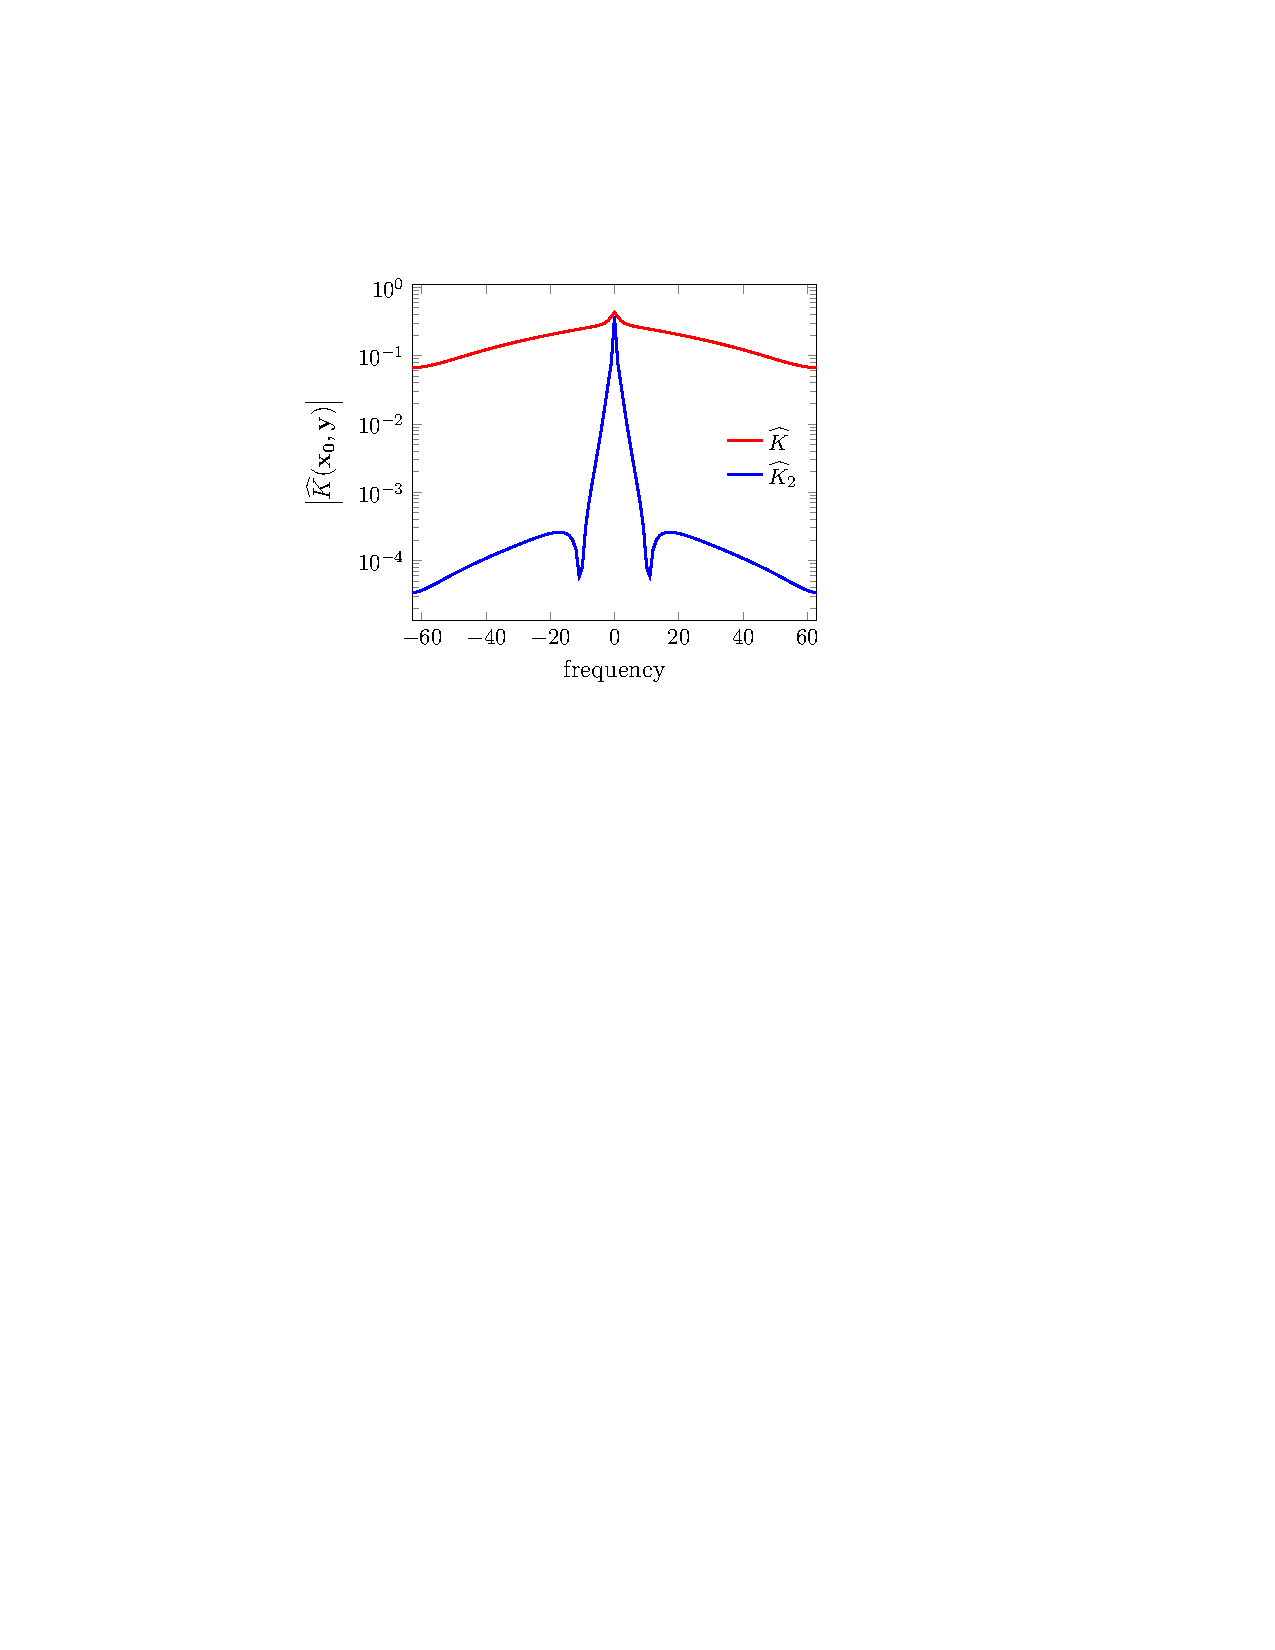
\includegraphics[width=2.5in]{figures/integrands}}
\vspace*{-13pt}
  \caption{{\footnotesize The Fourier modes of
  $K(\mathbf{x_0},\mathbf{y})$ and $K_2(\mathbf{x_0},\mathbf{y})$ where
  $|\mathbf{x_0}| = 0.99$ and $\mathbf{y} \in \partial\Omega$, and
  $\Omega$ is the unit circle. The trapezoid rule applied to the red
  integrand has large amounts of error, but the trapezoid rule is much
  more accurate when applied to the blue integrand. Since the difference
  between the red and blue curves can be accurately computed with the
  barycentric quadrature rule, the quadrature error applied to layer
  potentials for the screen Laplace equation will be uniformly bounded
  in $\Omega$.}}
\label{fig:integrands}
\end{wrapfigure}
Nearly touching bodies is ubiquitous in self-assembly of amphiphilic
particles, and this results in nearly-singular integrands. Quadrature
methods for these integrands has received a lot of attention in two and
three dimensions~\cite{alpert, kapur, sidi, duffy, bruno1, bruno2,
davis_1984, graglia_2008, hackbusch_sauter_1994, jarvenpaa_2003,
khayat_2005, schwab_1992, ying_2006, beale1, schwab_1992, ggq1, ggq2,
ggq3, helsing_2008a, helsing_tutorial_2012, klockner2013jcp, qbx2,
wala2019jcp, af2018sisc, siegel2018jcp, rachh2017jcp, ding2019arxiv,
bar2014}. The trapezoid rule is the workhorse for two-dimensional BIEs
since it achieves spectral accuracy when integrands are not
nearly-singular~\cite{tre-wei2014}. To address nearly-singular
integrands of two-dimensional BIEs, we will use a {\em barycentric
quadrature rule} that only requires a slight modification of the
trapezoid rule~\cite{ioa-pap-per1991}. In its current form, this method
requires the layer potential to satisfy Laplace or Stokes
equations~\cite{bar-wu-vee2015, chi-moo-qua2020}, but the PIs will
extend the method to layer potentials for the screened Laplace equation.
This will be done by recognizing that the fundamental solution of the
screened Laplace equation can be decomposed as $K(\mathbf{x},\mathbf{y})
= K_1(\mathbf{x},\mathbf{y}) + K_2(\mathbf{x},\mathbf{y})$, where
$K_1(\mathbf{x},\mathbf{y}) = -\log|\mathbf{x} - \mathbf{y}|$ and
$K_2(\mathbf{x},\mathbf{y}) = K(\mathbf{x},\mathbf{y}) + \log|\mathbf{x}
- \mathbf{y}|$. Then, layer potentials involving
$K_1(\mathbf{x},\mathbf{y})$ can be accurately computed with the
barycentric quadrature rule~\cite{ioa-pap-per1991}, and layer potentials
involving $K_2(\mathbf{x},\mathbf{y})$ can be accurately computed with
the trapezoid rule since the kernel is bounded for all $\mathbf{x}$ and
$\mathbf{y}$. The proposed method is demonstrated in
Figure~\ref{fig:integrands} where the amplitude of the Fourier modes of
$K(\mathbf{x_0},\mathbf{y})$ and $K_2(\mathbf{x_0},\mathbf{y})$ are
plotted. The quadrature error of the trapezoid rule is the sum of the
unresolved Fourier modes.


% ----------------------------------------------------------------------
\subsubsection{Eliminating contact with adaptive time stepping and
repulsion}
\label{subsec:timeStepping}

A numerical issue when simulating the self-assembly of amphiphilic
particles is avoiding particle collision. The hydrophobic attraction
potential drives the amphiphilic particles towards one another so to
minimize exposure to the solvent, and this leads to physical contact in
finite time. Such particle collisions in a dense rigid body suspension
is a great challenge and can be a bottleneck in large-scale simulations.
We propose two algorithms to remedy this computational challenge:
high-order adaptive time stepping and repulsion forces.

PI BQ developed a high-order adaptive time stepping method for
hydrodynamic suspensions~\cite{qua-bir2016} and it has served as a
robust method to simulate processes including mixing and adhesion in
suspensions~\cite{qua-vee-you2019, kab-qua-bir2017}. The method uses
a single-step high-order time stepping method and a computationally
cheap estimate of the error. The proposed work will use a spectral
deferred correction method~\cite{dut-gre-rok2000} since it iteratively
applies a low-order single-step method to achieve high-order accuracy.
To estimate the error, at each time step we will compute the total force
and torque of the system which is computationally cheap and physically
zero. PI BQ's experience is that error estimates based on physical
constraints such as force- and torque-free conditions appropriately
determine how the time step should be adjusted so that the dynamics are
resolved without the computational expense of techniques such as
embedded Runge-Kutta methods, step-doubling, and Richardson
extrapolation.

%
\begin{wrapfigure}[13]{r}{0.30\textwidth}
\centerline{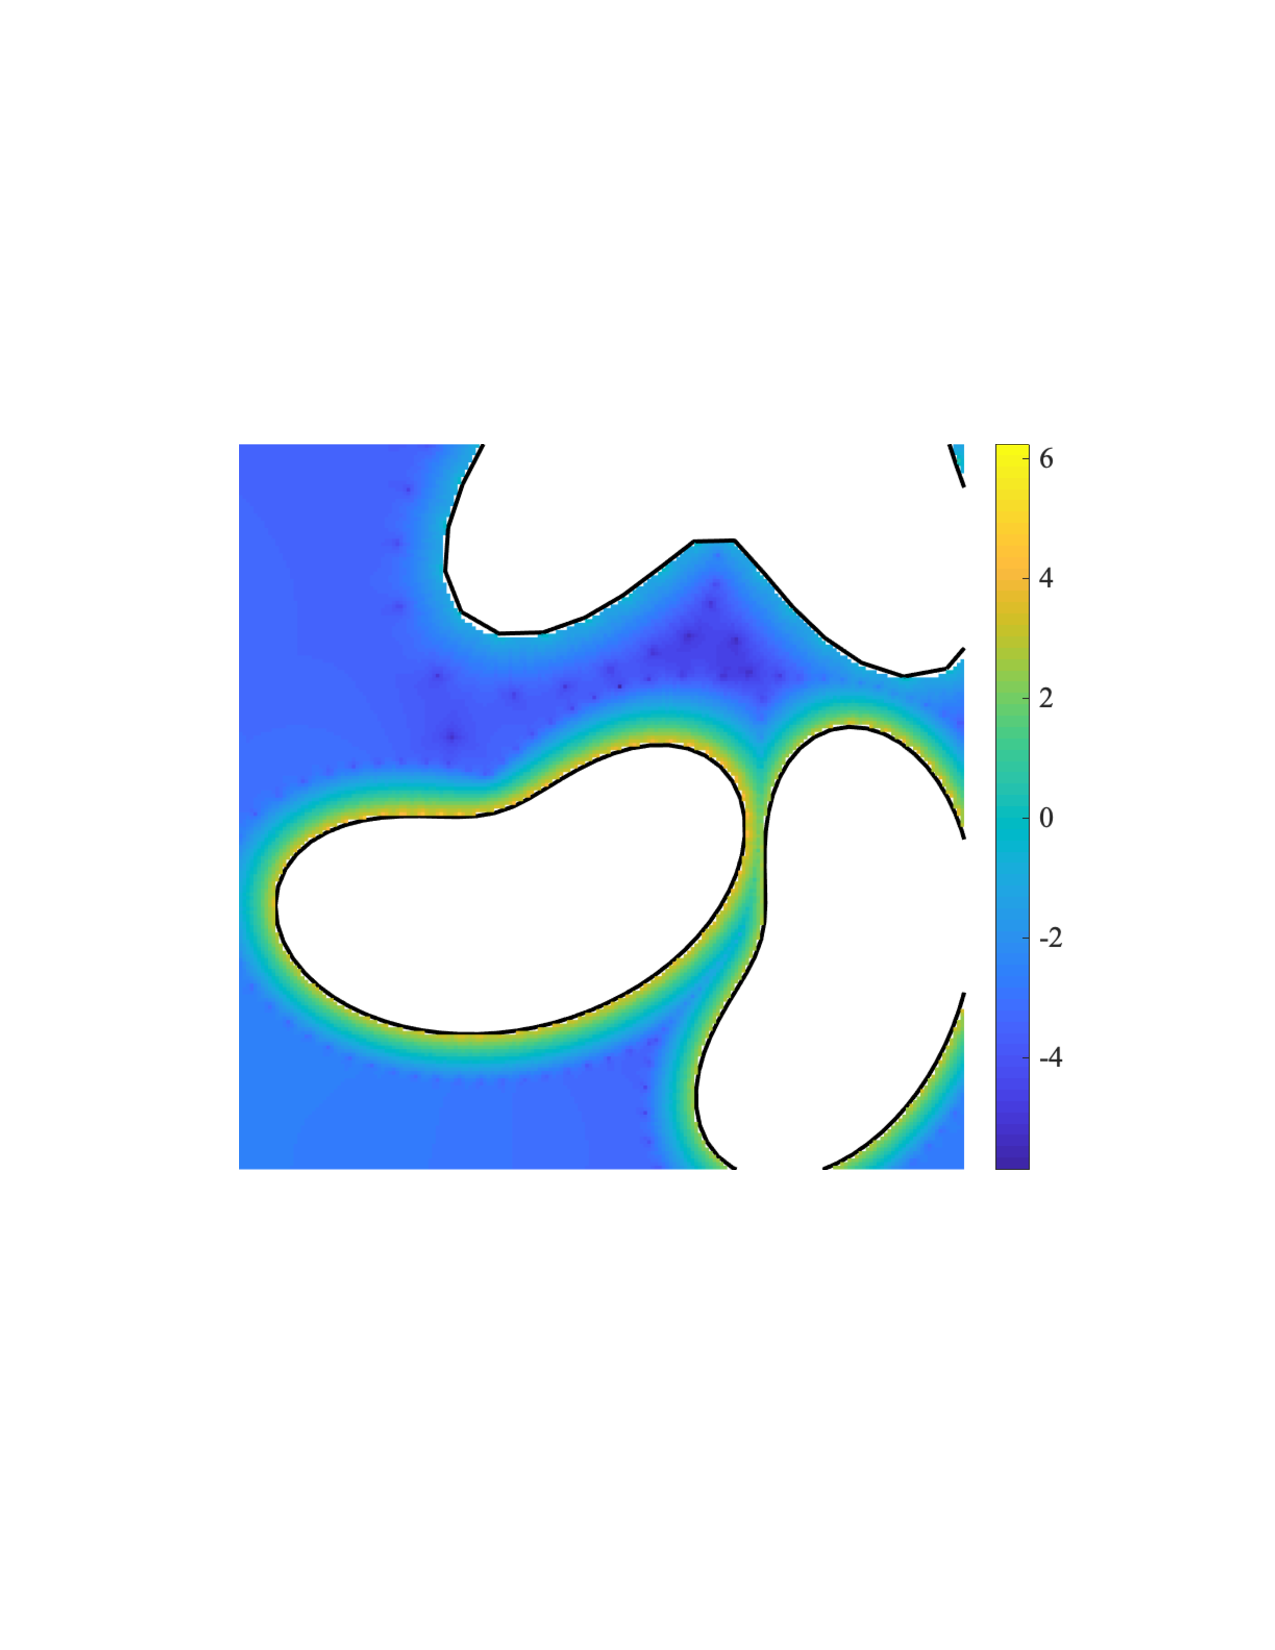
\includegraphics[width=0.30\textwidth]{figures/BIError.pdf}}
  \vspace{-8pt}
\caption{
\label{fig:bierror}  
\footnotesize The false color map shows how numerical quadrature of
  layer potentials loses accuracy near the particle boundaries.  The
  color bar is for $\log_{10}.$}
\end{wrapfigure}
%
Our previous work avoids contact by including a Lennard-Jones body
forces~\cite{Fu2018_SIAM}. Such a steep steric interaction at short
ranges introduces numerical stiffness and limits the time step size. To
remove this stiffness, we propose a geometry-based contact
method~\cite{har-pon-sor-zor2011}, and this method has been applied to
vesicle suspensions~\cite{lu-rah-zor2017} and rigid body suspensions in
two dimensions~\cite{bys-sha-qua2020} and three
dimensions~\cite{Yan2019}. These methods determine repulsion force by
solving a non-linear complementarity problem with a geometric constraint
that the configuration is non-overlapping. In this manner, contact is
avoided without the excessively small time steps required by stiff
Lennard-Jones forces.

%-------------------------------------------------------------------------------
\subsubsection{Novel reciprocal identities}
\label{subsec:reciprocal}
The force and torque formulas~\eqref{forceandtorque} require the
hydrophobic stress along the particle boundaries. Unfortunately,
layer potentials for $\nabla u$ involve hyper-singular integrals and
this introduces large amounts of quadrature error on the particle
boundaries (Figure~\ref{fig:bierror}). Therefore, it is useful to devise
reciprocal identities for the force and torque on body $i$ that does not
require integration along body $i$. One identity, that we have proved,
is
\begin{align}
    \label{eq:reciprocal}
{\bf F}_{\text{hydro},i} = \sum_{j \neq i} \int_{\partial P_i}[\boldsymbol{\sigma}_{ij} + \boldsymbol{\sigma}_{ji}]\boldsymbol{\nu}\,\dif S,\quad
{\bf G}_{\text{hydro},i} = \sum_{j \neq i} \int_{\partial P_i} ({\bf
  x}-\mathbf{a}_i) \times [\boldsymbol{\sigma}_{ij} +
  \boldsymbol{\sigma}_{ji}]\boldsymbol{\nu}\,\dif S, 
\end{align}
for $i=1,\ldots,N$. Here, $u_i$ is the solution of the screened Laplace
equation when only the contribution from particle $i$ is considered and
$\boldsymbol{\sigma}_{ij} = \rho^{-1} u_iu_j \mathbf{I} +
\rho\left((\nabla u_i \cdot \nabla u_j) \mathbf{I} - 2 \nabla u_i
\otimes \nabla u_j\right)$. Equation~\eqref{eq:reciprocal} does not
require knowledge of $\nabla u$ on the particle boundary, and this is
enormously beneficial for calculating the hydrophobic force and torque.

% ----------------------------------------------------------------------
\subsubsection{Fluctuating hydrodynamics}
\label{subsec:fluctuating}
Once algorithms that address quadrature, adaptive time stepping, and
contact are implemented, we will embark on incorporating fluctuating
hydrodynamics that are important even at scales of some amphiphilic
particles. Bao et al.~\cite{Bao17,Bao18} developed two-dimensional BIE
formulations for Brownian rigid bodies. To satisfy the covariance of the
rigid body velocities, they use an ill-conditioned first-kind integral
equation method. The proposed work will consider a layer potential
formulation that has much better conditioning properties. This strategy
was attempted in~\cite{Bao18}, but they claim that a necessary
regularization of the covariance matrix leads to a drastic loss of
accuracy in numerical fluctuation-dissipation balance. However, only one
regularization strategy was considered, and as PI BQ has shown in
previous work, the regularization choice significantly affects the
resulting physics~\cite{ong-chr-qua2017}. Therefore, different
regularization strategies will be investigated with the goal of
controlling the accuracy of the fluctuation-dissipation balance.


